\section{Pileup Epoch Comparison Study}
\label{sec:PileupEpochStudy}

The presence of pileup and how it is dealt with
is discussed in Section.~\ref{sec:pileup}.
After making the aforementioned corrections we verify that all effects
have been accounted for by comparing 2010 Data, 2011A Data, 2011B Data
(which contain progressively higher amounts of pileup events) as well as the
(default LO) W+jets Monte Carlo. As shown in Fig.~\ref{fig:PUEpochComp}, there are no
statistically significant discrepancies between the $M_{jj}$ distributions.

%%%%%%%
\begin{figure}[h!] {\centering
\unitlength=0.33\linewidth
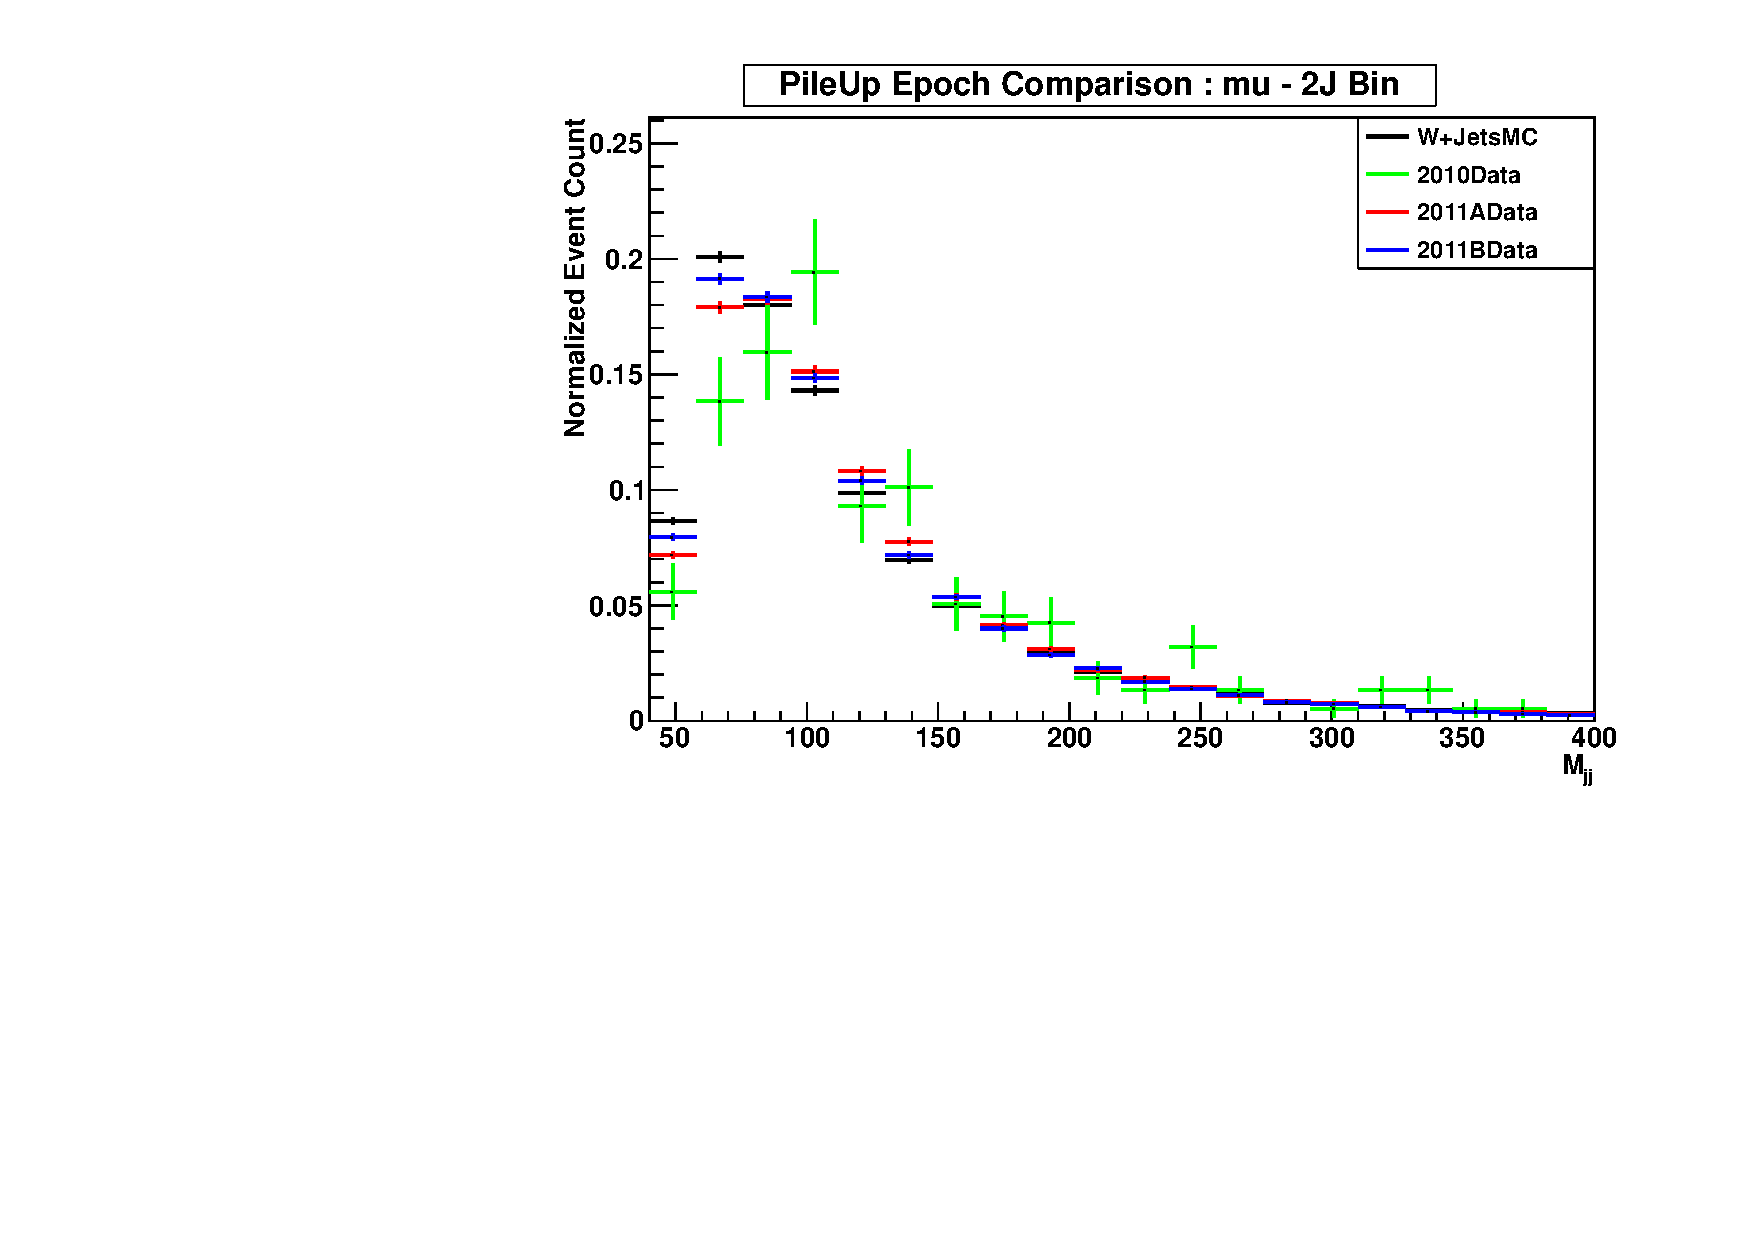
\includegraphics[width=0.48\textwidth]{figs/AdditionalStudies/PUEpochs_mu2J.pdf}
\put(-0.80,0.0){(a)} 
\unitlength=0.33\linewidth
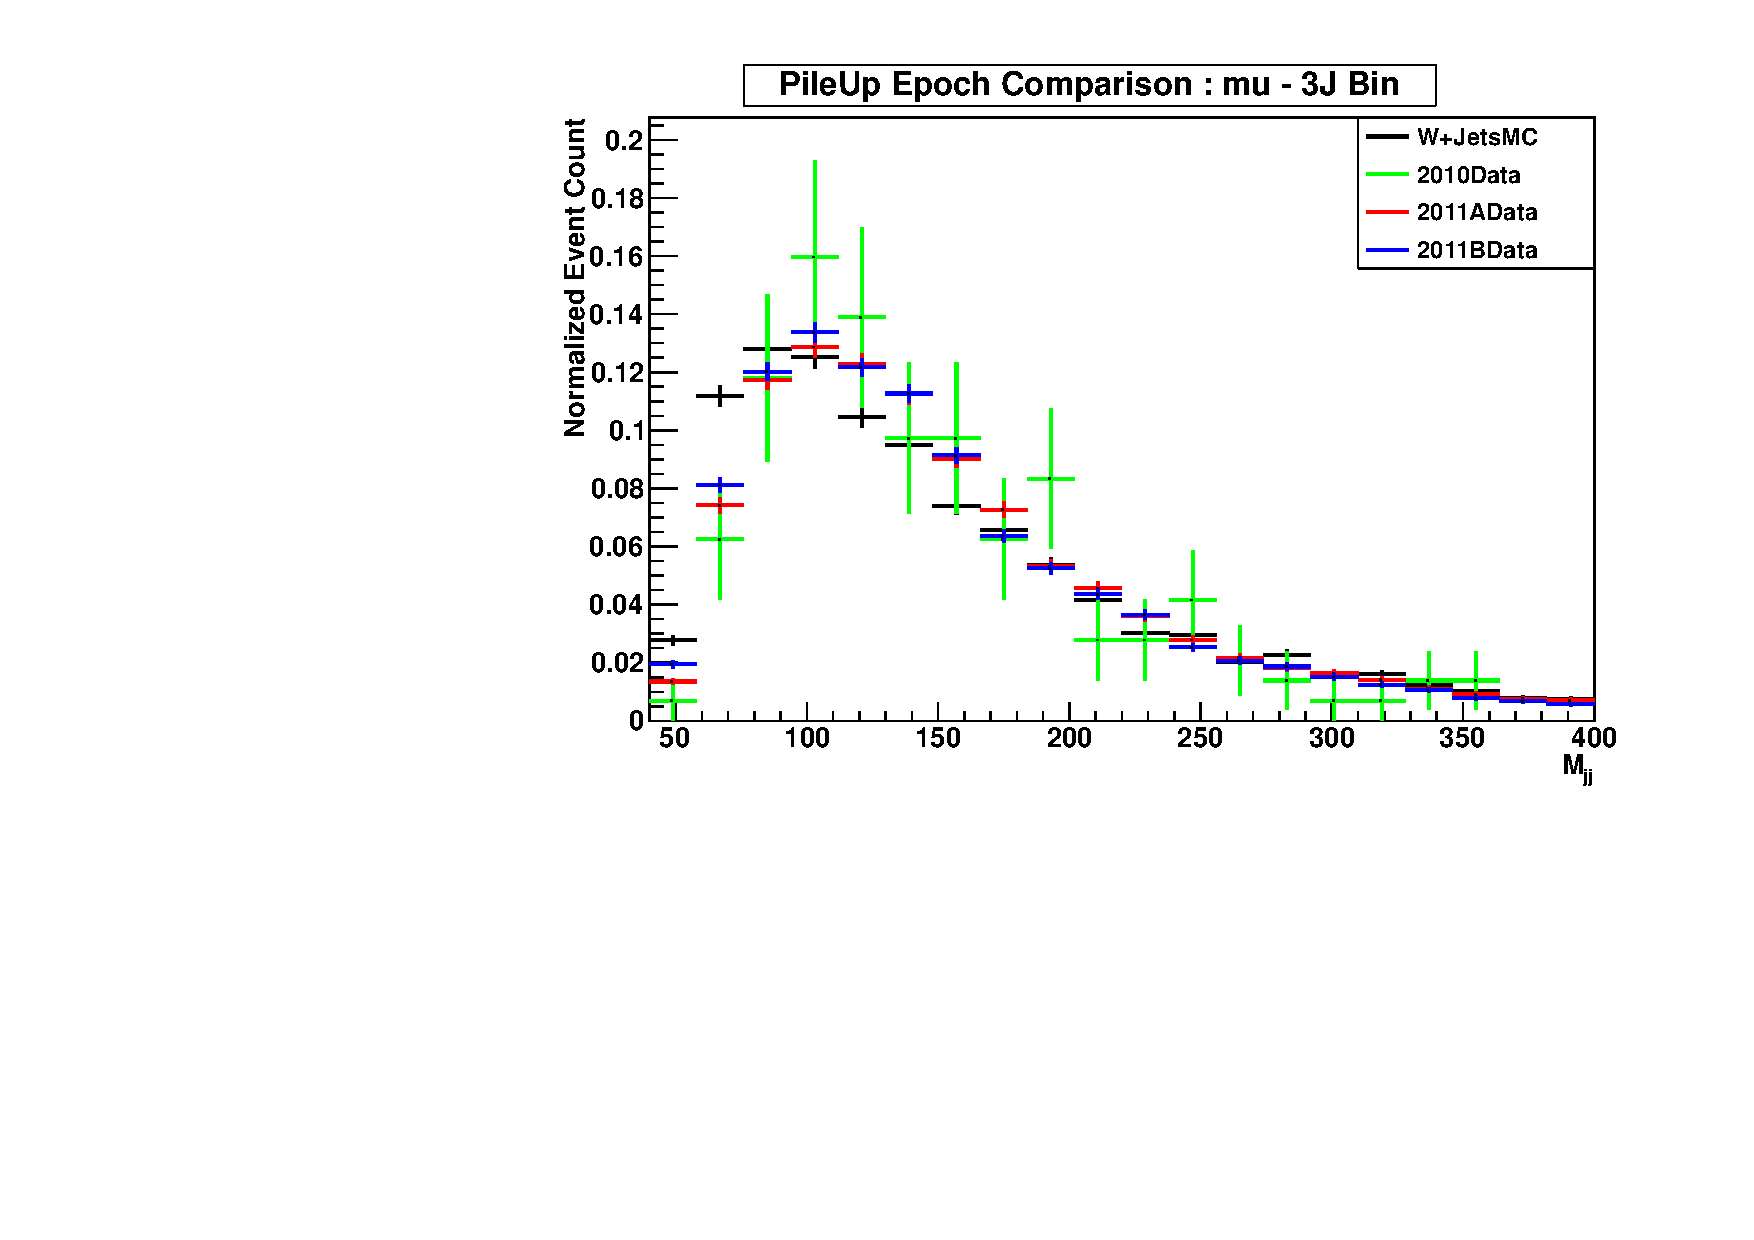
\includegraphics[width=0.48\textwidth]{figs/AdditionalStudies/PUEpochs_mu3J.pdf}
\put(-0.80,0.0){(b)} \\
\unitlength=0.33\linewidth
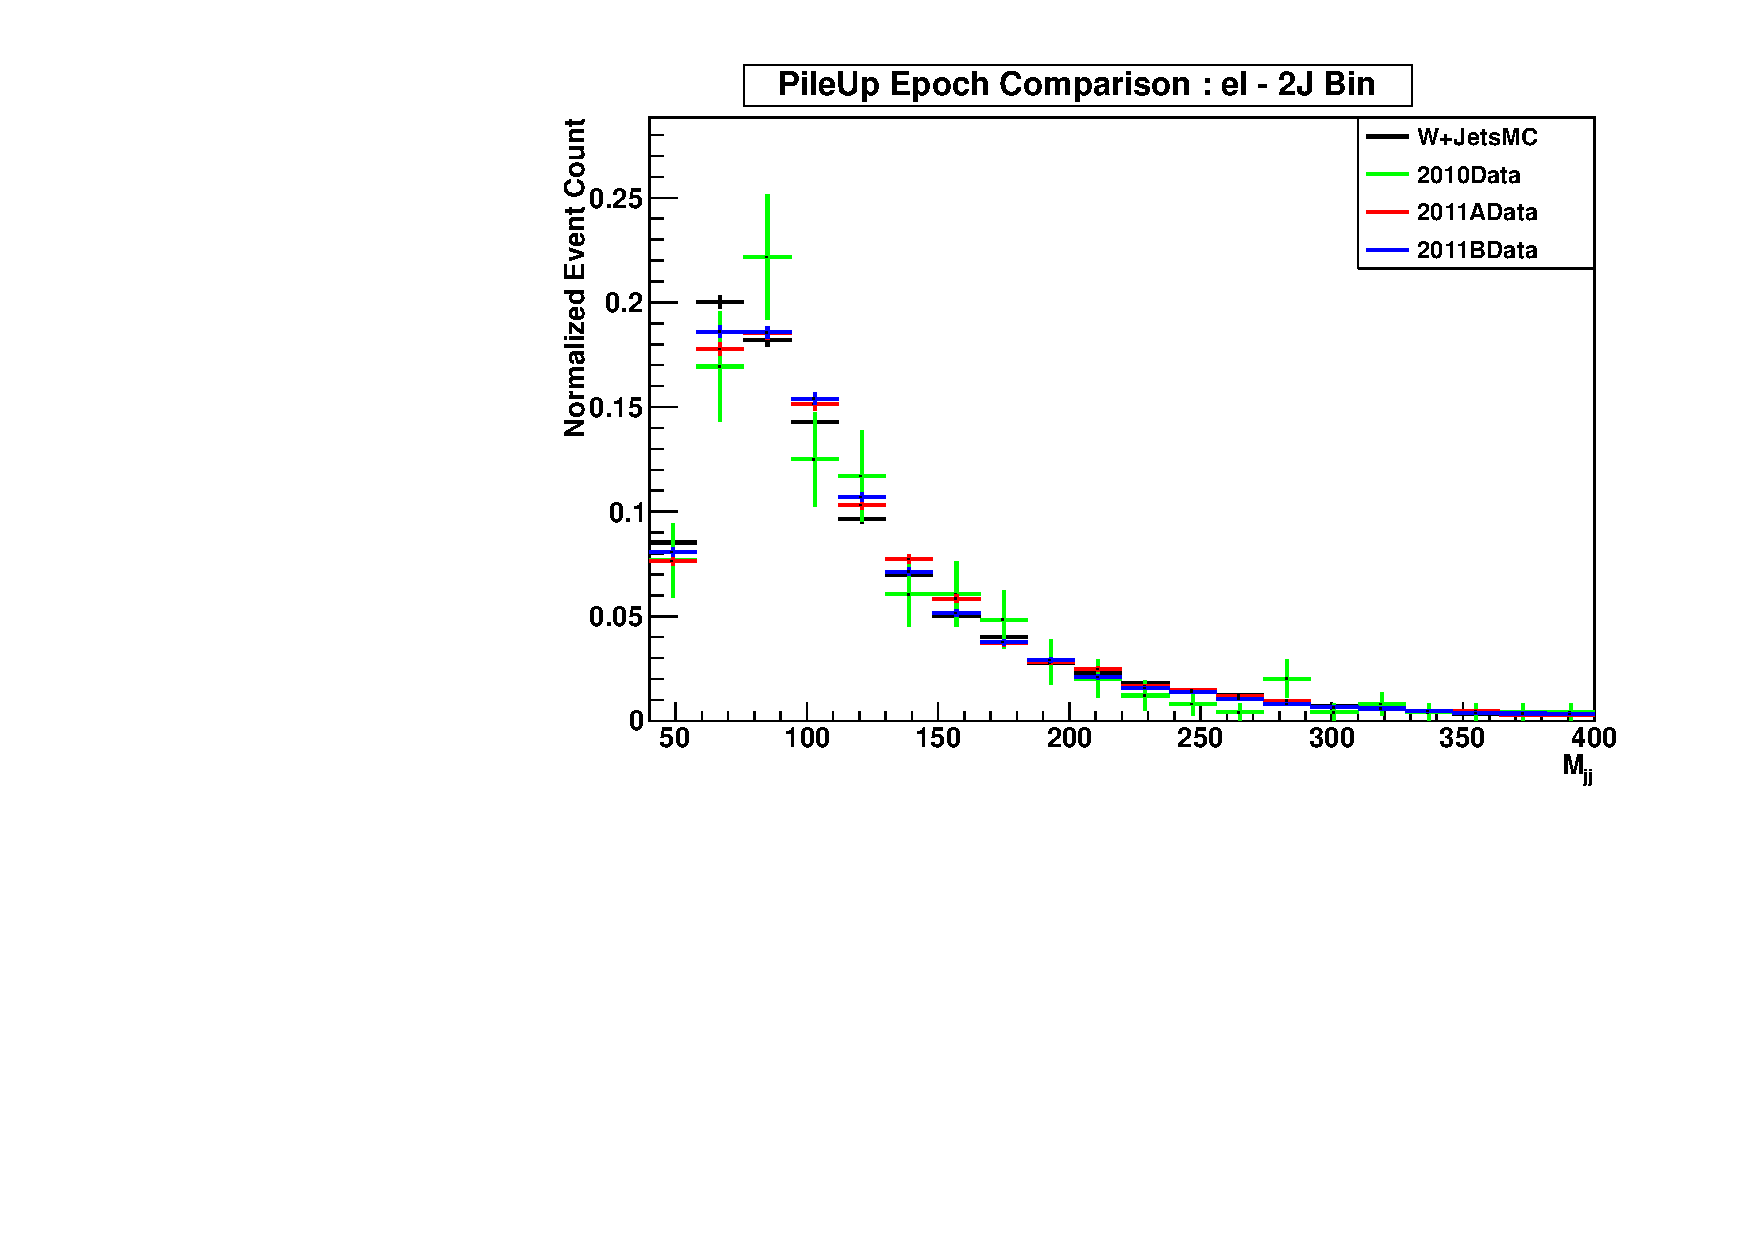
\includegraphics[width=0.48\textwidth]{figs/AdditionalStudies/PUEpochs_el2J.pdf}
\put(-0.80,0.0){(c)} 
\unitlength=0.33\linewidth
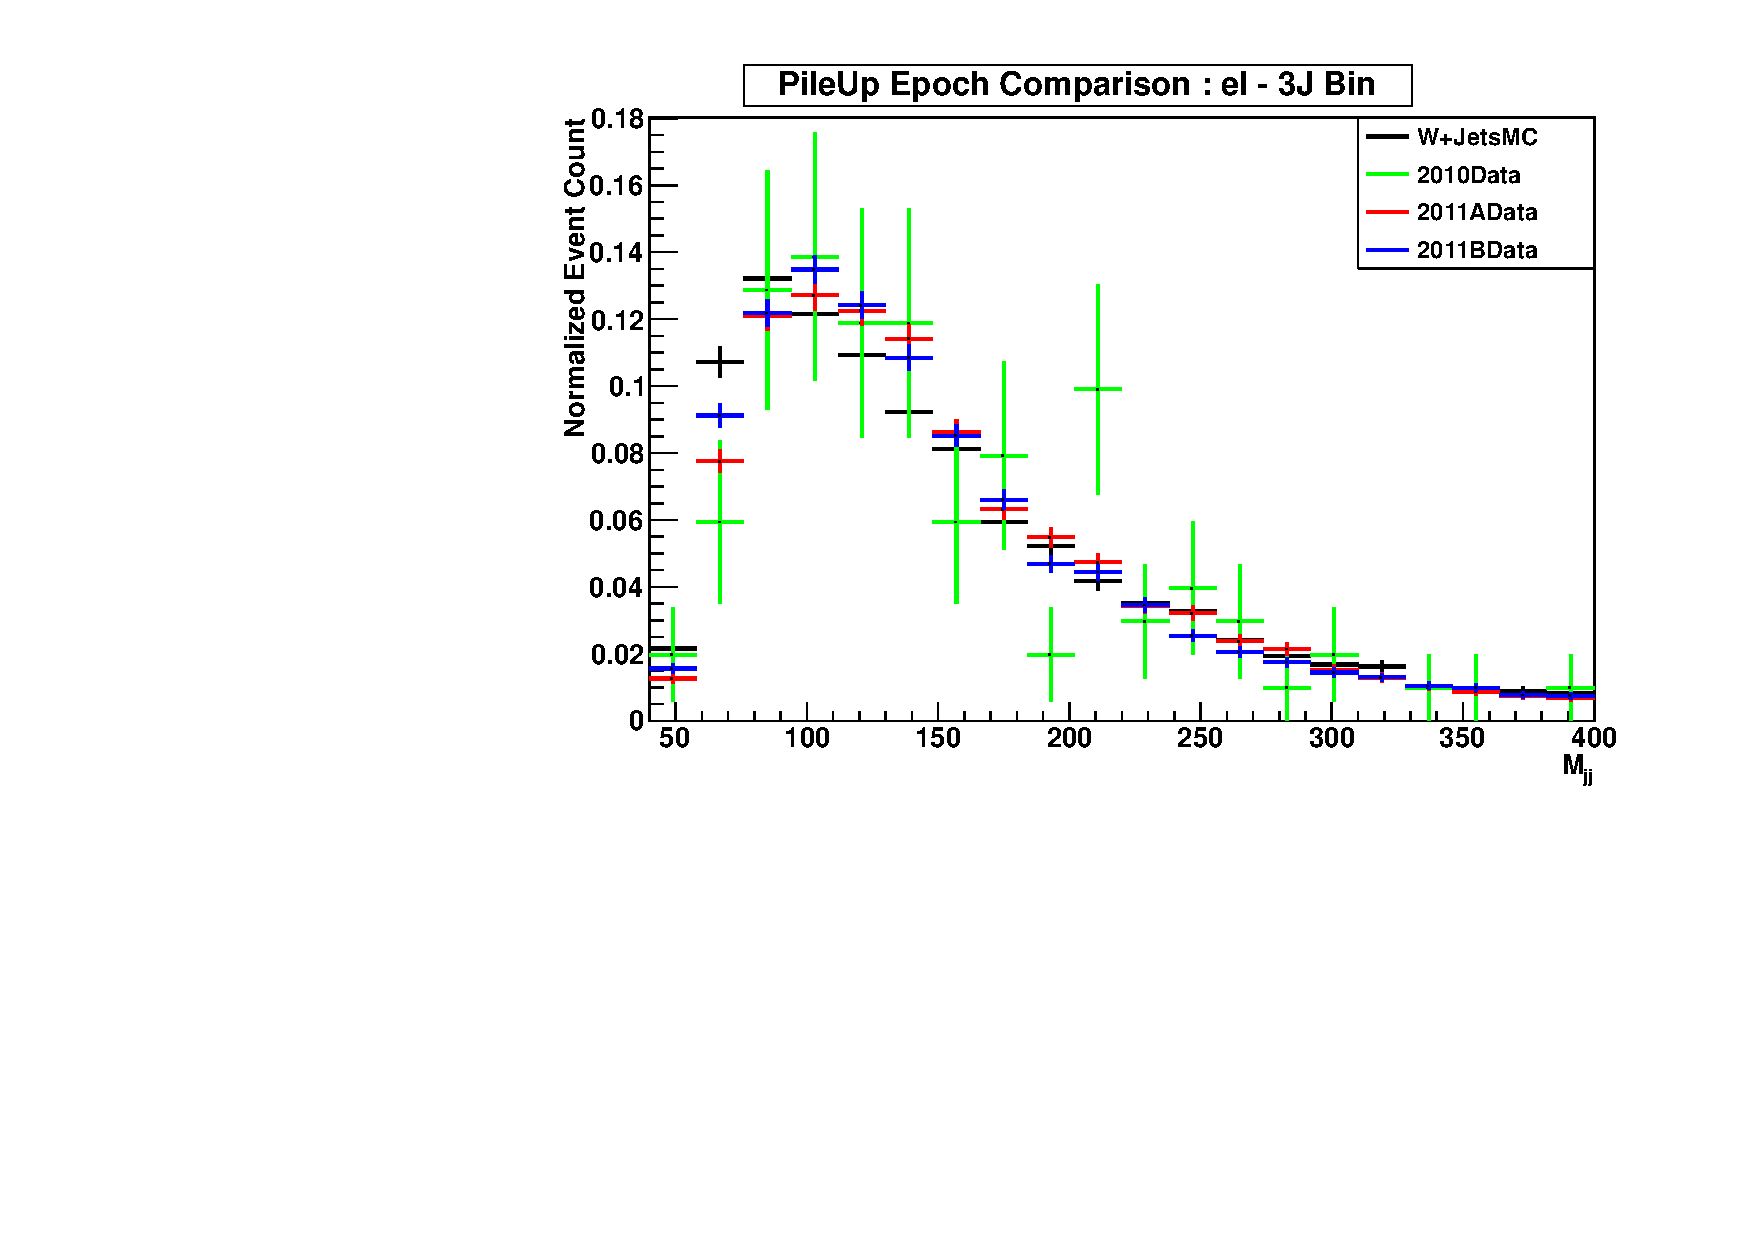
\includegraphics[width=0.48\textwidth]{figs/AdditionalStudies/PUEpochs_el3J.pdf}
\put(-0.80,0.0){(d)} 
\caption{Comparison between epochs with differing amounts of pileup for: (a) muons - 2-jet bin, (b) muons - 3-jet bin, (c) electrons - 2-jet bin, (d) electrons - 3-jet bin.} 
\label{fig:PUEpochComp}
}
\end{figure}
%%%%%%%
